\documentclass[a4paper]{article}
\usepackage{times}
\usepackage[utf8]{inputenc}
\usepackage{selinput}
\usepackage{upquote}
\usepackage[margin=2cm, rmargin=4cm, tmargin=3cm]{geometry}
\usepackage{tcolorbox}
\usepackage{xspace}
\usepackage[french]{babel}
\usepackage{url}
\usepackage{hyperref}
\usepackage{fontawesome5}
\usepackage{marginnote}
\usepackage{ulem}
\usepackage{tcolorbox}
\usepackage{graphicx}
%\usepackage[top=Bcm, bottom=Hcm, outer=Ccm, inner=Acm, heightrounded, marginparwidth=Ecm, marginparsep=Dcm]{geometry}


\newtcolorbox{Example}[1]{colback=white,left=20pt,colframe=slideblue,fonttitle=\bfseries,title=#1}
\newtcolorbox{Solutions}[1]{colback=white,left=20pt,colframe=green,fonttitle=\bfseries,title=#1}
\newtcolorbox{Conseils}[1]{colback=white,left=20pt,colframe=slideblue,fonttitle=\bfseries,title=#1}
\newtcolorbox{Warning}[1]{colback=white,left=20pt,colframe=warning,fonttitle=\bfseries,title=#1}

\setlength\parindent{0pt}

  %Exercice environment
  \newcounter{exercice}
  \newenvironment{Exercice}[1][]
  {
  \par
  \stepcounter{exercice}\textbf{Question \arabic{exercice}:} (\faClock \enskip \textit{#1})
  }
  {\bigskip}
  

% Title
\newcommand{\titre}{\begin{center}
  \section*{Algorithmes et Pensée Computationnelle}
\end{center}}
\newcommand{\cours}[1]
{\begin{center} 
  \textit{#1}\\
\end{center}
  }


\newcommand{\exemple}[1]{\newline~\textbf{Exemple :} #1}
%\newcommand{\attention}[1]{\newline\faExclamationTriangle~\textbf{Attention :} #1}

% Documentation url (escape \# in the TP document)
\newcommand{\documentation}[1]{\faBookOpen~Documentation : \href{#1}{#1}}

% Clef API
\newcommand{\apikey}[1]{\faKey~Clé API : \lstinline{#1}}
\newcommand{\apiendpoint}[1]{\faGlobe~Url de base de l'API \href{#1}{#1}}

%Listing Python style
\usepackage{color}
\definecolor{slideblue}{RGB}{33,131,189}
\definecolor{green}{RGB}{0,190,100}
\definecolor{blue}{RGB}{121,142,213}
\definecolor{grey}{RGB}{120,120,120}
\definecolor{warning}{RGB}{235,186,1}

\usepackage{listings}
\lstdefinelanguage{texte}{
    keywordstyle=\color{black},
    numbers=none,
    frame=none,
    literate=
           {é}{{\'e}}1
           {è}{{\`e}}1
           {ê}{{\^e}}1
           {à}{{\`a}}1
           {â}{{\^a}}1
           {ù}{{\`u}}1
           {ü}{{\"u}}1
           {î}{{\^i}}1
           {ï}{{\"i}}1
           {ë}{{\"e}}1
           {Ç}{{\,C}}1
           {ç}{{\,c}}1,
    columns=fullflexible,keepspaces,
	breaklines=true,
	breakatwhitespace=true,
}
\lstset{
    language=Python,
	basicstyle=\bfseries\footnotesize,
	breaklines=true,
	breakatwhitespace=true,
	commentstyle=\color{grey},
	stringstyle=\color{slideblue},
  keywordstyle=\color{slideblue},
	morekeywords={with, as, True, False, Float, join, None, main, argparse, self, sort, __eq__, __add__, __ne__, __radd__, __del__, __ge__, __gt__, split, os, endswith, is_file, scandir, @classmethod},
	deletekeywords={id},
	showspaces=false,
	showstringspaces=false,
	columns=fullflexible,keepspaces,
	literate=
           {é}{{\'e}}1
           {è}{{\`e}}1
           {ê}{{\^e}}1
           {à}{{\`a}}1
           {â}{{\^a}}1
           {ù}{{\`u}}1
           {ü}{{\"u}}1
           {î}{{\^i}}1
           {ï}{{\"i}}1
           {ë}{{\"e}}1
           {Ç}{{\,C}}1
           {ç}{{\,c}}1,
    numbers=left,
}

\newtcbox{\mybox}{nobeforeafter,colframe=white,colback=slideblue,boxrule=0.5pt,arc=1.5pt, boxsep=0pt,left=2pt,right=2pt,top=2pt,bottom=2pt,tcbox raise base}
\newcommand{\projet}{\mybox{\textcolor{white}{\small projet}}\xspace}
\newcommand{\optionnel}{\mybox{\textcolor{white}{\small Optionnel}}\xspace}
\newcommand{\advanced}{\mybox{\textcolor{white}{\small Pour aller plus loin}}\xspace}
\newcommand{\auto}{\mybox{\textcolor{white}{\small Auto-évaluation}}\xspace}


\usepackage{environ}
\newif\ifShowSolution
\NewEnviron{solution}{
  \ifShowSolution
	\begin{Solutions}{\faTerminal \enskip Solution}
		\BODY
	\end{Solutions}
  \fi}


  \usepackage{environ}
  \newif\ifShowConseil
  \NewEnviron{conseil}{
    \ifShowConseil
    \begin{Conseils}{\faLightbulb \quad Conseil}
      \BODY
    \end{Conseils}

    \fi}

    \usepackage{environ}
  \newif\ifShowWarning
  \NewEnviron{attention}{
    \ifShowWarning
    \begin{Warning}{\faExclamationTriangle \quad Attention}
      \BODY
    \end{Warning}

    \fi}
  

%\newcommand{\Conseil}[1]{\ifShowIndice\ \newline\faLightbulb[regular]~#1\fi}


\usepackage{array}
\usepackage{blindtext}
\usepackage{multicol}
\newcolumntype{C}[1]{>{\centering\let\newline\\\arraybackslash\hspace{0pt}}m{#1}}

\begin{document}
% Change the following values to true to show the solutions or/and the hints
\ShowSolutiontrue
\ShowConseiltrue
\titre
\cours{Consolidation 2}

Les exercices de cette série sont une compilation d'exercices semblables à ceux vus lors des semaines précédentes. Le but de cette séance est de consolider les connaissances acquises lors des travaux pratiques des dernière semaines.\\

% Exercice complexité - Maeva
\begin{Exercice}[10 minutes] \textbf{Complexité} \\
	Analysez la complexité pour les deux codes suivants. Est-ce la même pour fun() et fun2() ? Pourquoi ?
    	\lstinputlisting{resources/ex1_enonce.py}

	% Solutions complexité - Maeva
	\begin{solution}
	Non, ils n'ont pas la même complextié. Fun() a une complexité de O(n*n) car il s'agit de deux boucles imbriquées. En revanche, fun2() a une 	complexité de O(n+n) car il s'agit de deux boucles indépendante.  
	\end{solution}
\end{Exercice}

% Exercice complexité - Maeva
\begin{Exercice}[10 minutes]\textbf{Complexité}\\
	Quel est la complexité de ce code ?
   	 \lstinputlisting{resources/ex2_enonce.py}
	 % Exercice complexité - Maeva
	 \begin{solution}
		%TODO 
	\end{solution}
\end{Exercice}

% Exercice nombres impaire - Maeva
\begin{Exercice}[10 minutes] \\
	Ecrivez un programme python qui permet d’imprimer tous les nombres impairs à partir de 1 jusqu’à un nombre n défini par l’utilisateur (qui doit être supérieur à 1) :
	Exemple : si n = 6, résultat attendu : 1, 3, 5
% Solutions nombres impaire - Maeva
	\begin{solution}
   		 \lstinputlisting{solutions/exercise3.py}
	\end{solution}
\end{Exercice}

% Exercice arbres binaires - Maeva
\begin{Exercice}
	Lesquels (ou lequel) de ces arbres est un arbre binaire (binary tree) ? Donnez leur hauteur (height).
	\begin{figure}[h!]
        		\centering
       	 	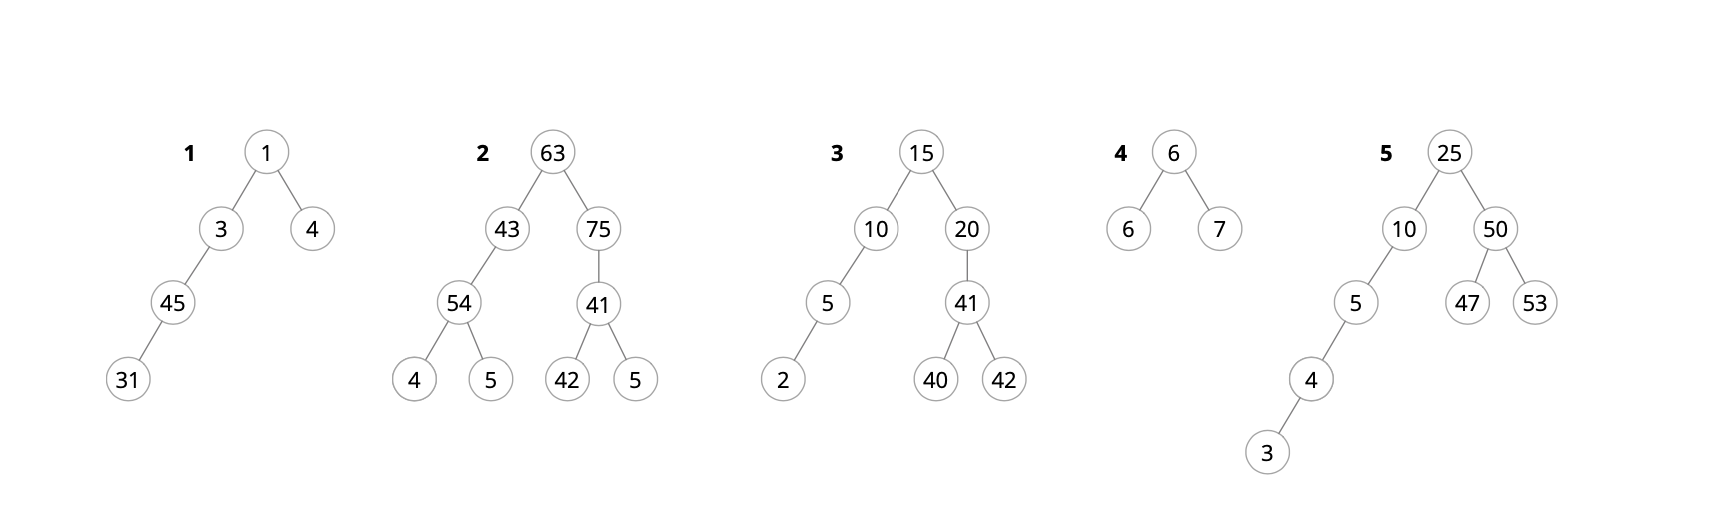
\includegraphics[width=10cm]{resources/exercice5.png}
    	\end{figure}
	% Solution arbres binaires - Maeva
	\begin{solution}
		1. Il ne s'agit pas d'un arbre binaire car il n'y a pas decondition qui est remplie à chaque noeuds. Sa hauteur est de 3.\\
		2. Il ne s'agit pas d'un arbre binaire car il n'y a pas de condition qui est remplie à chaque noeuds. Sa hauteur est de 3.\\
		3. Il s'agit d'un arbre binaire car une condition peut être appliquée à chaque noeud. Sa hauteur est de 3.\\
		4. Il s'agit d'un arbre binaire car une condition peut être appliquée à chaque noeud. Sa hauteur est de 1.\\
		5. Il s'agit d'un arbre binaire car une condition peut être appliquée à chaque noeud. Sa hauteur est de 4.\\
	\end{solution}
\end{Exercice}


% Exercice complexité - Etienne
\begin{Exercice}[10 minutes]\textbf{Trie complexité}\\
	Trier la liste de fonctions suivante selon leur croissance assymptotique:
	\begin{equation}
		n^{\sqrt{n}}, n\cdot log(n), n^{1/log(n)}, log(log(n)), \sqrt{n}, 3^{n}/{n^5}, 2^n
	\end{equation}
	
	% Solutions complexité - Etienne
	\begin{solution}
		\begin{itemize}
			\item D'abord la constante : $n^{1/log(n)} = (2^{log(n)})^{1/log(n)}$
			\item Ensuite le $log(log(n))$
			\item Puis $n^{\sqrt{n}} = 2^{\sqrt{n}\cdot log_2(n)}$
			\item Puis $2^n$
			\item Enfin  $3^{n}/{n^5}$
		\end{itemize}
	\end{solution}
\end{Exercice}


% Exercice théorique - Etienne
\begin{Exercice}[20 minutes]\textbf{Théorie}\\
	\begin{enumerate}
		\item Donner en pseudo code un algorithme ayant une complexité temporelle de O(log n) qui prend comme argument un tableau trié A[1, ..., n] de n nombres et une clé k et qui retourne "OUI" si A contient k et "NON" sinon.
		\item Quelle est la hauteur maximum et la hauteur minimale d'un arbre binaire de recherche ayant n éléments ? Quel arbre est meilleur ? Justifier.
		\item Considerer l'arbre binaire suivant : \\
		\begin{figure}[h!]
        			\centering
       	 		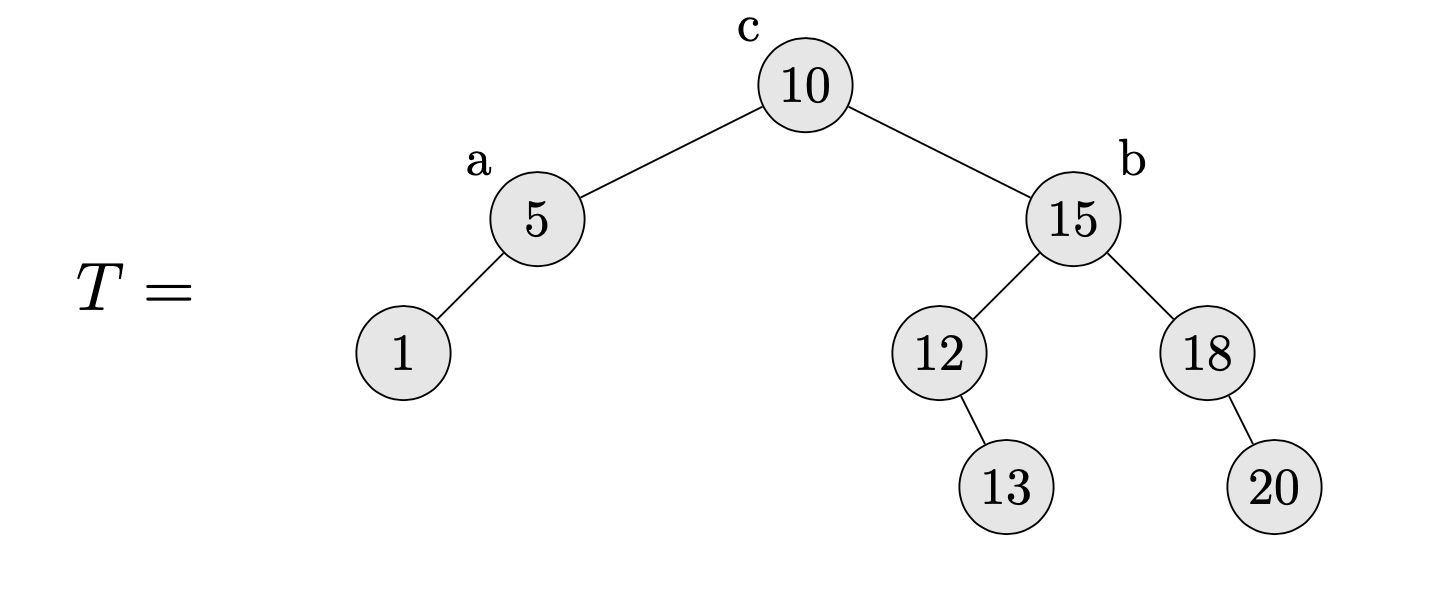
\includegraphics[width=10cm]{resources/exoArbreBinEnonce.png}
	    	\end{figure}
		Dessiner les arbres obtenus après executions de chacune des opérations suivantes (chaque opération est exécutée en commençant par l'arbre ci-dessus - les opérations ne sont pas exécutée séquentiellement).
		\begin{enumerate}
			\item \textsc{Tree-Insert}(T, z) avec z.key = 0
			\item \textsc{Tree-Insert}(T, z) avec z.key = 17
			\item \textsc{Tree-Insert}(T, z) avec z.key = 14
			\item \textsc{Tree-Delete}(T, a)
			\item \textsc{Tree-Delete}(T, b)
			\item \textsc{Tree-Delete}(T, c)
		\end{enumerate}


	\end{enumerate}
	% Solution exercice théorique - Etienne
	\begin{solution}
		\begin{enumerate}
			\item Etant donné que les nombres du tableau A sont triés, nous utilisons l'algorithme de recherche binaire. L'algorithme de recherche binaire  prend comme argument un tableau A, une clé k, des indices p et q et retourne "OUI" si A[p . . . q]  contient la clé k et "NON" autrement. Comme A[p . . . q] est trié, nous pouvons comparer k avec l'élément du milieu mid = $\lfloor(p+q)//2\rfloor$  et : \\
				\begin{itemize}
					\item Si A[mid] = k return "OUI" \\
					\item Si A[mid] $>$ k, alors cherchons k dans le tableau A[p . . . (mid-1)] en appelant récursivement l'algorithme \textsc{Binary-Search}(A, k, p, mid-1) \\
					\item Si A[mid] $<$ k, alors cherchons k dans le tableau A[(mid + 1) . . . q] en appelant récursivement l'algorithme \textsc{Binary-Search}(A, k, mid+1, q)\\
				\end{itemize}
				The pseudo-code of the procedure is as follows:
				\lstinputlisting{solutions/exerciseTheorieBinarySearch.py}
				Note that we solve the original problem by calling \textsc{Binary-Search}(A, k, 1, n).
			\item Hauteur minimale et maximale d'un arbre binaire.
				\begin{itemize}
					\item La hauteur maximum d'un arbre binaire est atteinte quand l'arbre n'est constitué d'une seule branche. \\
						%\begin{figure}[h!]
        						%	\centering
       	 					%	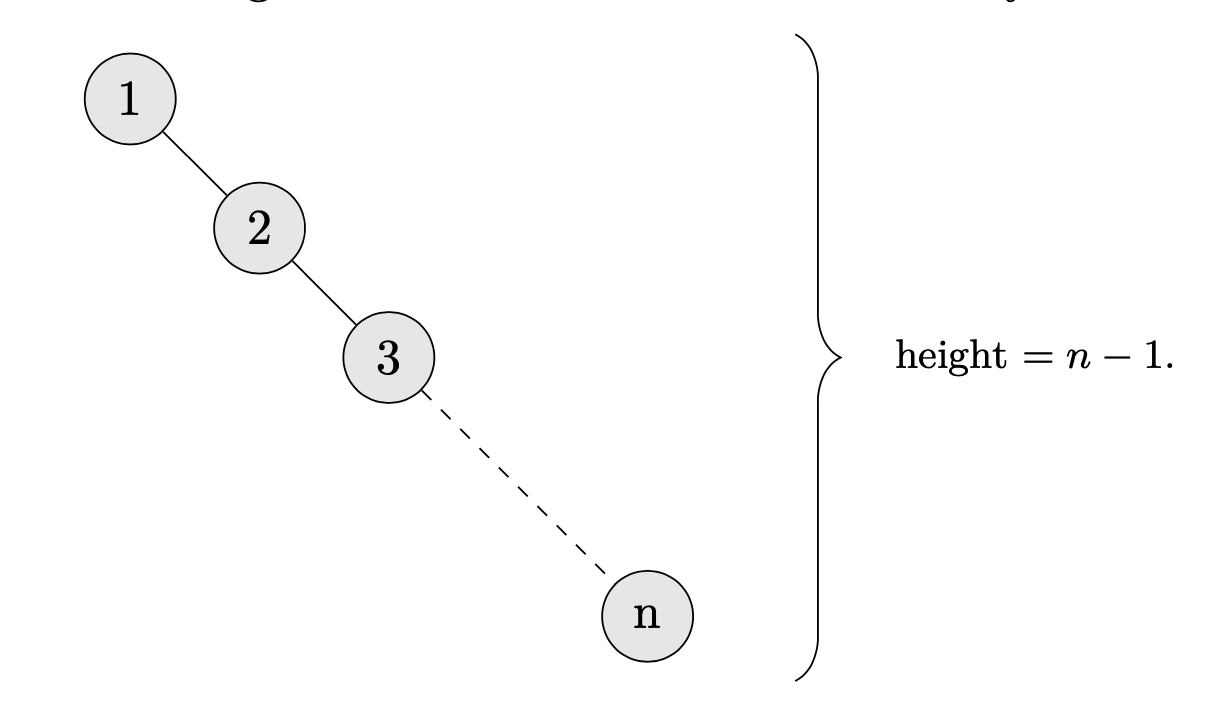
\includegraphics[width=6cm]{solutions/maxHeight.png}
	    					%\end{figure}
					\item La hauteur minimum est atteinte lorsque l'arbre binaire est "complet" : nous ne pouvons pas ajouter un noeud sans augmenter la hauteur de l'arbre hauteur de un. \\
						%\begin{figure}[h!]
        						%	\centering
       	 					%	\includegraphics[width=6cm]{solutions/min_height.png}
	    					%\end{figure}
				\end{itemize}
			\item Après execution de chaque opération, nous obtenons:
				\begin{enumerate}
					\item Figure A : \textsc{Tree-Insert}(T, z) avec z.key = 0
						%\begin{figure}[h!]
        						%	\centering
       	 					%	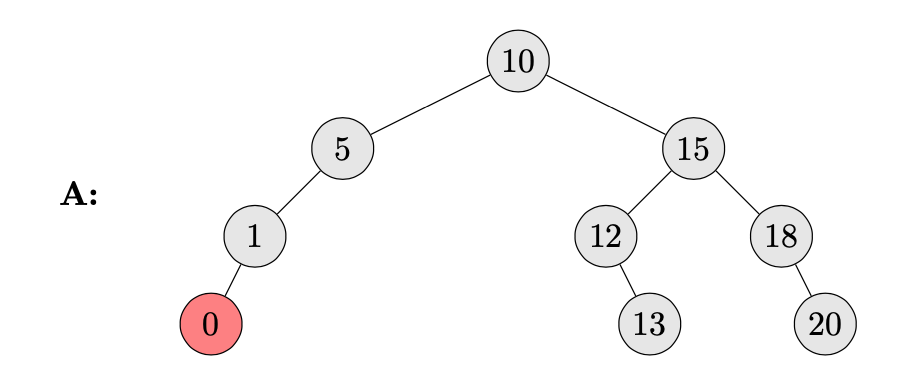
\includegraphics[width=6cm]{solutions/exoBTFigA.png}
	    					%\end{figure}
					\item Figure B : \textsc{Tree-Insert}(T, z) avec z.key = 17
						%\begin{figure}[h!]
        						%	\centering
       	 					%	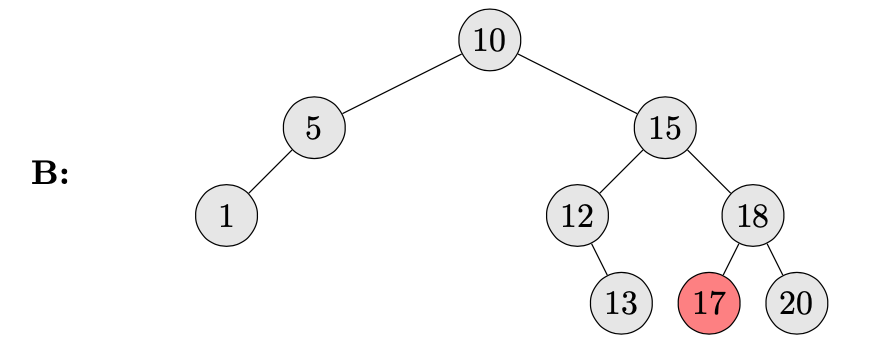
\includegraphics[width=6cm]{solutions/exoBTFigB.png}
	    					%\end{figure}
					\item Figure C: \textsc{Tree-Insert}(T, z) avec z.key = 14
						%\begin{figure}[h!]
        						%	\centering
       	 					%	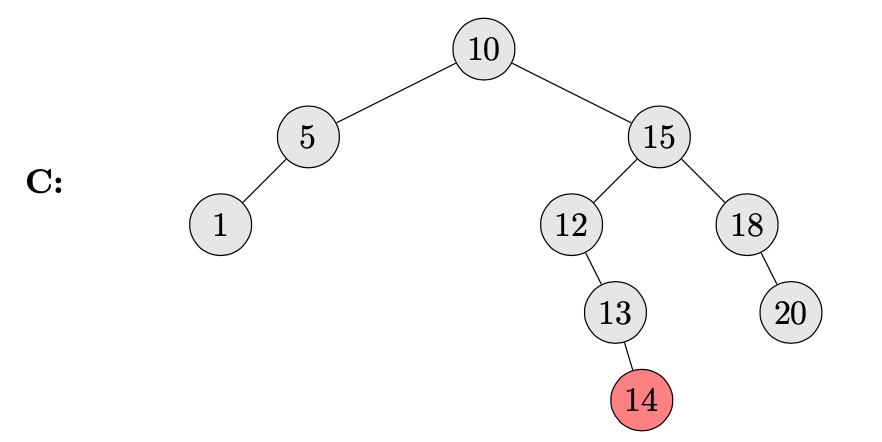
\includegraphics[width=6cm]{solutions/exoBTFigC.png}
	    					%\end{figure}
					\item Figure D : \textsc{Tree-Delete}(T, a)
						%\begin{figure}[h!]
        						%	\centering
						%	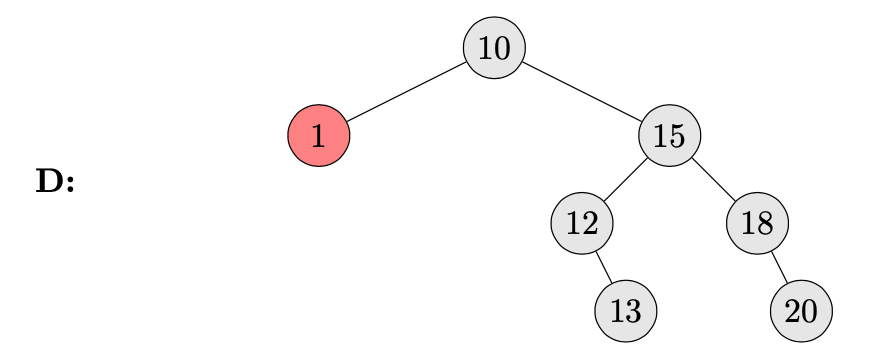
\includegraphics[width=6cm]{solutions/exoBTFigD.png}
	    					%\end{figure}
					\item Figure E : \textsc{Tree-Delete}(T, b)
						%\begin{figure}[h!]
        						%	\centering
       	 					%	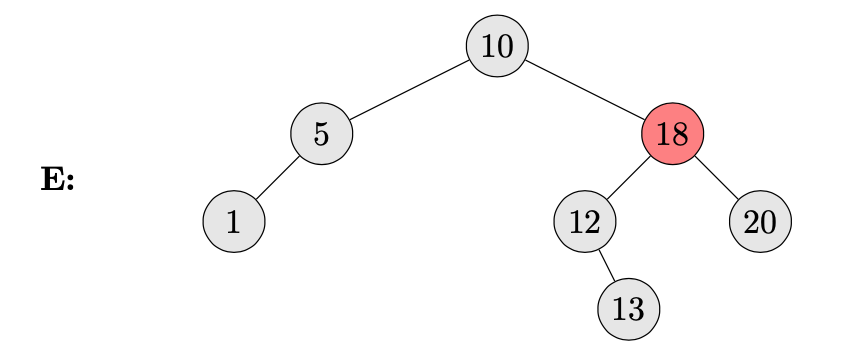
\includegraphics[width=6cm]{solutions/exoBTFigE.png}
	    					%\end{figure}
					\item Figure F : \textsc{Tree-Delete}(T, c)
						%\begin{figure}[h!]
        						%	\centering
       	 					%	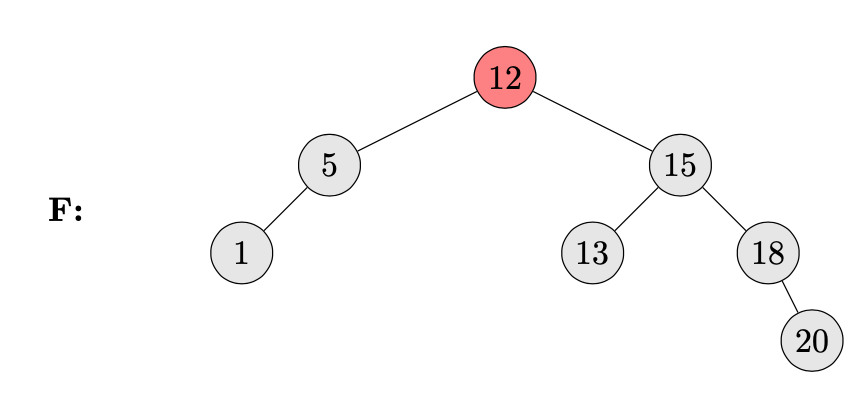
\includegraphics[width=6cm]{solutions/exoBTFigF.png}
	    					%\end{figure}
			\end{enumerate}
		\end{enumerate}
	\end{solution}
\end{Exercice}


% Exercice BFS Papier - Sarra
\begin{Exercice}[5 minutes]\textbf{Breadth-First Search algorithm : Papier
}\\
\\
	Le but du Breadth-first search (BFS) ou parcours en largeur est d'explorer le graphe à partir d’un sommet donné (sommet de départ ou sommet source). \\
	
	Appliquez l’algorithme de BFS au graphe suivant :\\

	\begin{figure}[h!]
        		\centering
       	 	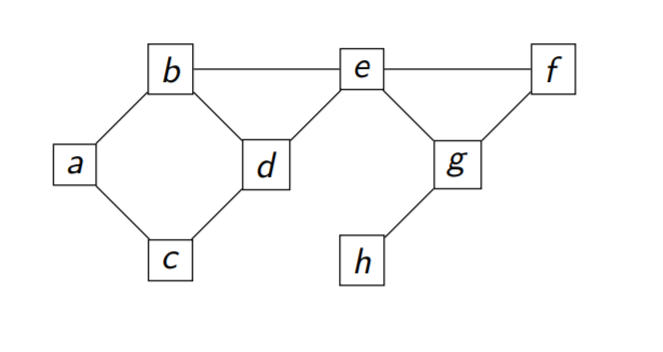
\includegraphics[]{resources/exerciceBFS.png}
	\end{figure}


	% Solution BFS - Sarra
	\begin{solution}
		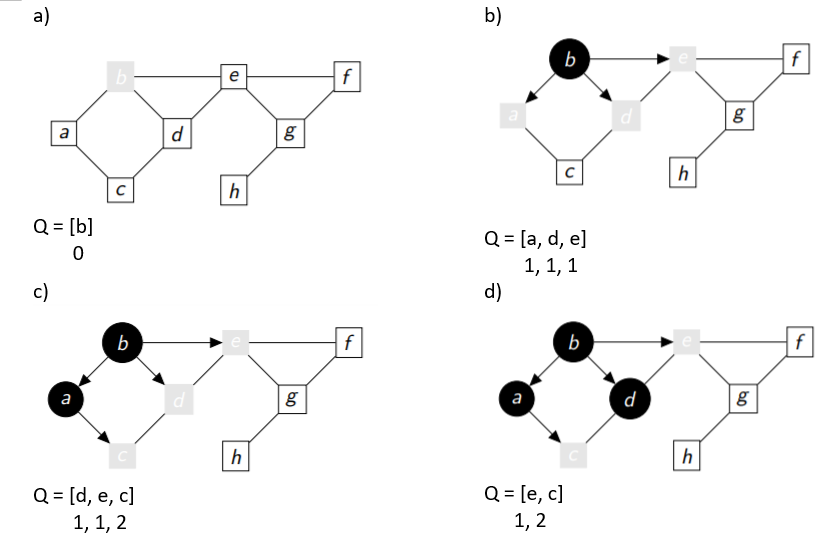
\includegraphics[width=10cm]{solutions/BFS1.PNG}\\
		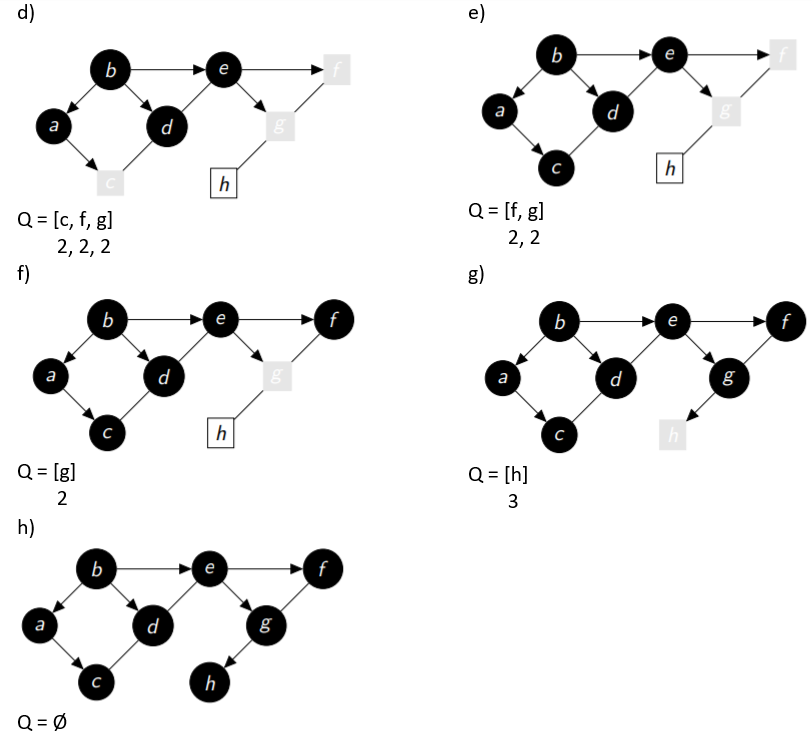
\includegraphics[width=10cm]{solutions/BFS2.PNG}\\
 		Ci-dessous l'arborescence associée au parcours.\\
		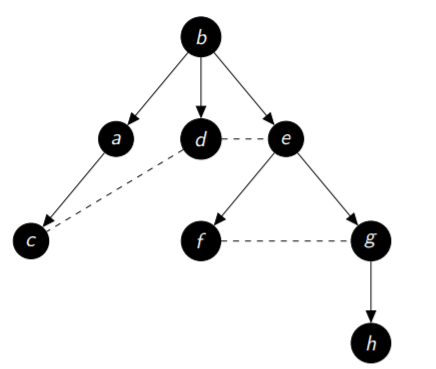
\includegraphics[]{solutions/BFS3.PNG}\\
		L’ordre de parcours est : ligne après ligne (de la racine vers les feuilles) et
		de gauche à droite pour une ligne.
	\end{solution}
\end{Exercice}

\end{document}